\begin{figure}[h!]
\textbf{Tema d'Esame di Febbraio 2017}\\ \\
Sapendo che la resistenza $R8$ è attraversata da una corrente $i_8 = 0.20 A$, si calcoli la corrente che attraversa $R3. R8 = 10 \Omega, R1 = R2 = R3 = 5.0 \Omega , R4 = 12 \Omega , R5 = 15 \Omega $.
\begin{center}
		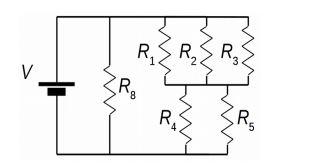
\includegraphics[scale=1.1]{ES5/FEB052017.jpg}
	\end{center}
\end{figure}

\begin{figure}[h!]
\textbf{Tema d'Esame di Giugno 2017}\\ \\
 Si determini il valore della resistenza $R_x$ del circuito mostrato nella figura sotto a sinistra. La differenza di potenziale fornita dalla batteria è $3 V$, la corrente i3 che scorre nella resistenza $R3$ è pari a $0.1 A$ ed i valori delle altre resistenze nel circuito
sono $R1 = R2 = 5 \Omega ,R3 = R4 = 10 \Omega$.
\begin{center}
		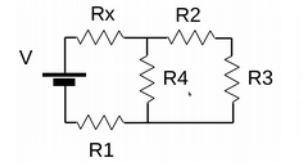
\includegraphics[scale=1.1]{ES5/GIU052017.jpg}
	\end{center}
\end{figure}

\begin{figure}[h!]
\textbf{Tema d'Esame di Settembre 2017}\\ \\
Trovare le correnti $i_1, i_2 , i_3$ nei tre rami del circuito qui sotto.
$R1 = 4.0 \Omega, R2 = 6.0 \Omega, R3 = 3.0 \Omega$ ed $ E 1 = 1.5 V,  E 2 = 3.0 V$.
\begin{center}
		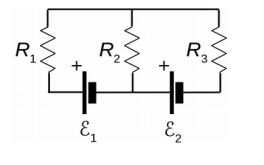
\includegraphics[scale=1.1]{ES5/SET052017.jpg}
	\end{center}
\end{figure}